% Appendix A

\chapter{Additional evaluation results} % Main appendix title

\label{AppendixA} % For referencing this appendix elsewhere, use \ref{AppendixA}

\lhead{Appendix A. \emph{Additional evaluation results}} % This is for the header on each page - perhaps a shortened title

\begin{figure}[htbp]
	\centering
		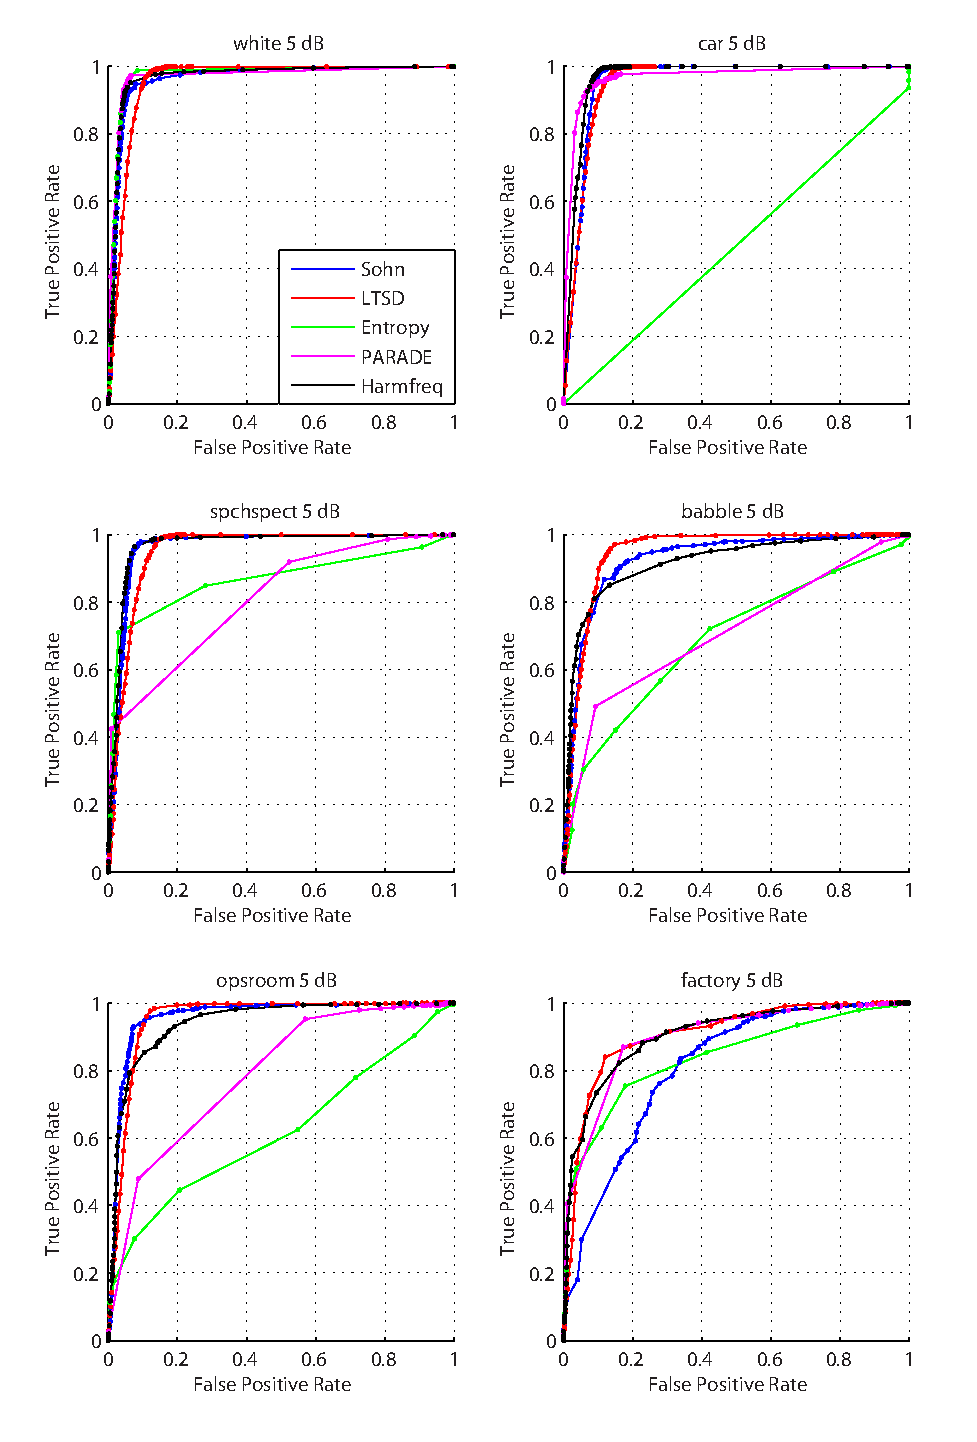
\includegraphics[width=1.0\columnwidth]{Figures/Chapter4/5dBh.pdf}
		\rule{37em}{0.5pt}
	\caption[ROC curves of the evaluated algorithms \emph{with} hang-over under 5 dB SNR]{ROC curves of the evaluated VAD algorithms \emph{with} hang-over under 5 dB SNR}
	\label{fig:5dBh}
\end{figure}

\begin{figure}[htbp]
	\centering
		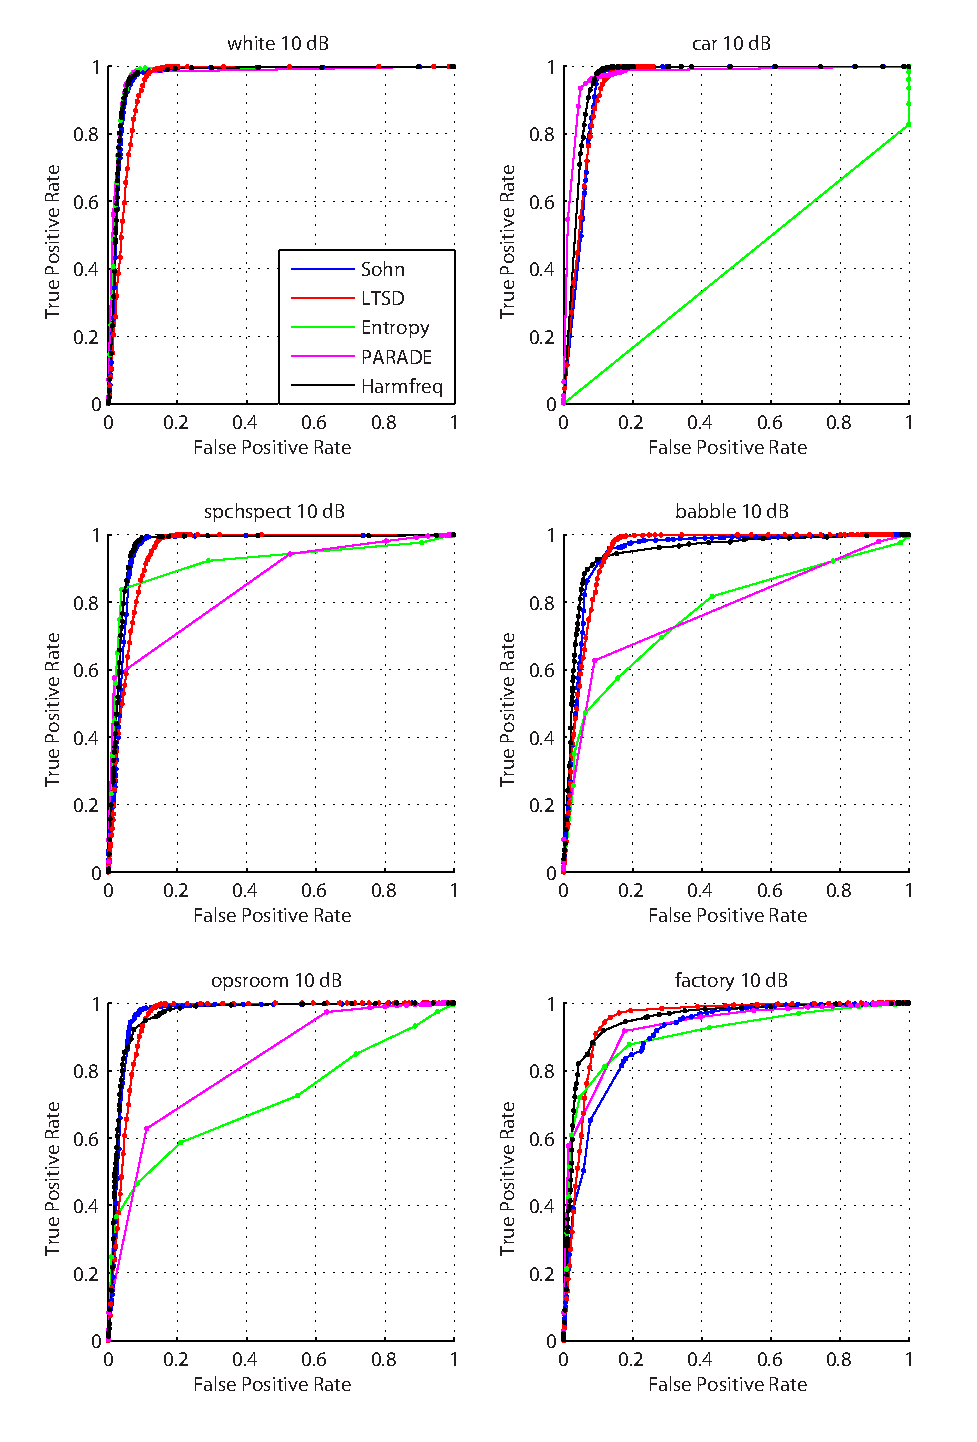
\includegraphics[width=1.0\columnwidth]{Figures/Chapter4/10dBh.pdf}
		\rule{37em}{0.5pt}
	\caption[ROC curves of the evaluated algorithms \emph{with} hang-over under 10 dB SNR]{ROC curves of the evaluated VAD algorithms \emph{with} hang-over under 10 dB SNR}
	\label{fig:10dBh}
\end{figure}

\begin{figure}[htbp]
	\centering
		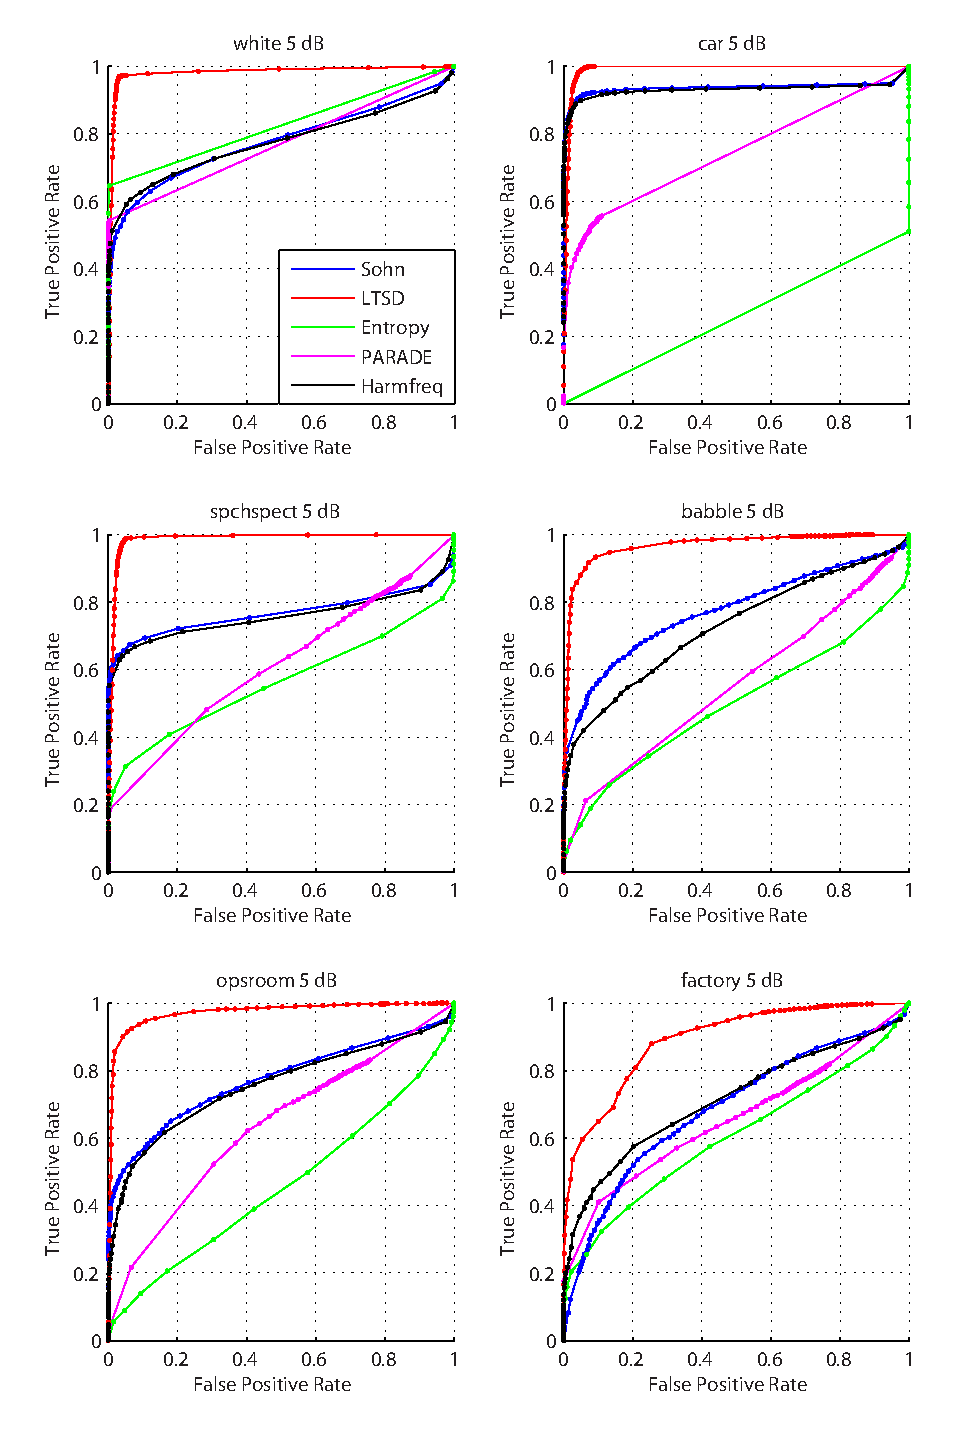
\includegraphics[width=1.0\columnwidth]{Figures/Chapter4/5dBnoh.pdf}
		\rule{37em}{0.5pt}
	\caption[ROC curves of the evaluated algorithms \emph{without} hang-over under 5 dB SNR]{ROC curves of the evaluated VAD algorithms \emph{without} hang-over under 5 dB SNR}
	\label{fig:5dBnoh}
\end{figure}

\begin{figure}[htbp]
	\centering
		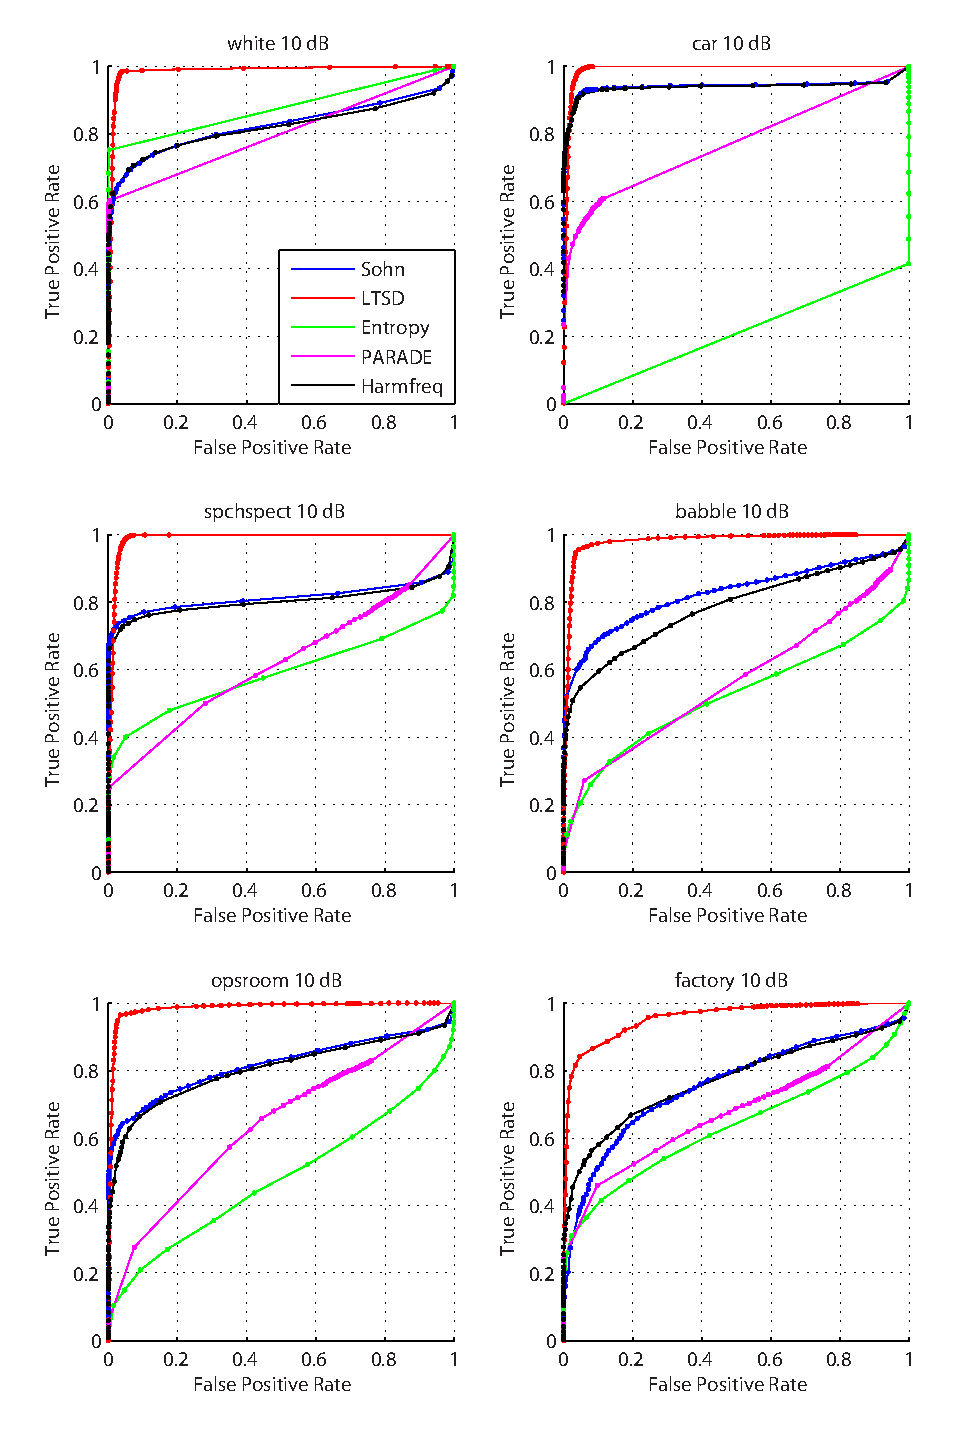
\includegraphics[width=1.0\columnwidth]{Figures/Chapter4/10dBnoh.pdf}
		\rule{37em}{0.5pt}
	\caption[ROC curves of the evaluated algorithms \emph{without} hang-over under 10 dB SNR]{ROC curves of the evaluated VAD algorithms \emph{without} hang-over under 10 dB SNR}
	\label{fig:10dBnoh}
\end{figure}